\textbf{7-1} 【题1】如力图7-1-1，质量为 $m$ 、劲度系数为 $k$ 的弹簧振子放在光滑的水平面上，其平衡位置在 $O$ 点，其圆频率 $\omega = 0.5\pi \mathrm{rad}\cdot \mathrm{s}^{-1}$ 。另一质量亦为 $m$ 的质点放在光滑曲面的 $A$ 点， $AB$ 间高度差 $h = 0.20\mathrm{m}$ ，质点由 $A$ 点滑到 $B$ 点所需时间 $t_{AB} = 1.5\mathrm{s}, OB$ 之间的距离 $l = 6.0\mathrm{m}$ 。现将弹簧振子向左压缩到 $x_0 = 2.0\mathrm{m}$ 处自由释放，同时释放 $A$ 处的质点 $m$ ，两个质点相遇作完全非弹性碰撞后粘在一起，发生碰撞时弹簧作用力可略。若从碰撞开始计时，试求系统振动的数学表达式。（取 $g = 10\mathrm{m / s^2}$ ）。

\begin{center}
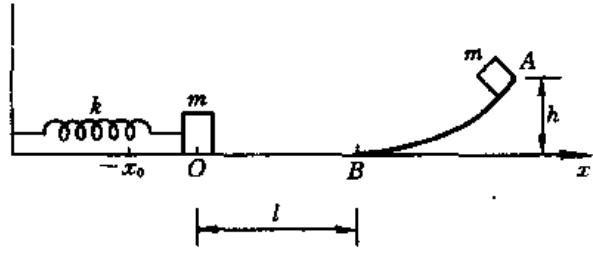
\includegraphics[width=0.3\textwidth]{figures/力图7-1-1.jpg}
\end{center}
\vfill

\textbf{7-2} 【题2】如力图7-2-1,某液体的密度随深度线性地增加,液体表面的密度为 $\rho_{0}$ , 深度为 D 处的密度为 $2\rho_{0}$ , 一密度为 $2\rho_{0}$ 的小球在深度为 $\frac{D}{2}$ 处从静止释放. 忽略液体的阻力. 试求小球的振动表达式.

\begin{center}
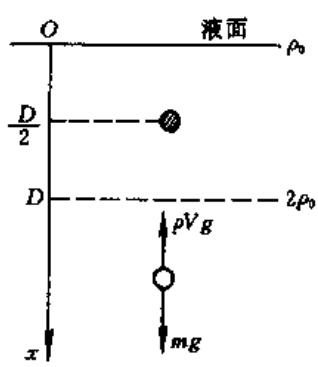
\includegraphics[width=0.2\textwidth]{figures/力图7-2-1.jpg}
\end{center}
\vfill

\newpage
\textbf{7-3} 【题3】如力图7-3-1,两个完全相同的圆柱状滚轮在水平面内平行放置,各绕自身的轴线按图示方向等角速转动,两轴线之间的距离为2l.在两滚轮上平放一块重量为G的均匀木板,木板与滚轮之间的摩擦系数为 $\mu$ .若木板重心偏离两轴中心位置一个微小的距离,试描述木板的运动.
\begin{center}
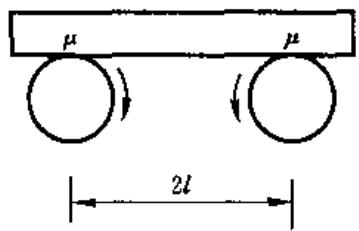
\includegraphics[width=0.25\textwidth]{figures/力图7-3-1.jpg}
\end{center}
\vfill

\textbf{7-4} 【题4】牛顿曾证明：一个均匀球壳，对球壳内物质的万有引力为零，而对球壳外物质的万有引

力不为零, 并且其作用就相当于球壳的质量都集中到球心那样(参看力学第三章题11). 如力图7-4-1所示, 设想沿地球直径开凿一条贯通地球的隧道, 将一小球从洞口由静止释放, 试求小球到达隧道另一洞口所用的时间. 已知地球的半径为 $R$ , 质量为 $M$ , 设地球的质量均匀分布.
\vfill

\newpage
\textbf{7-5} 【题5】如力图7-5-1，在倾角为 $\theta$ 的斜面上有一劲度系数为 $k$ 的弹簧，一端固定，另一端与质量为 $m$ 的实心圆柱体的轴连接，圆柱体在斜面上作纯滚动。忽略轴承的摩擦。试求振动周期。

\begin{center}
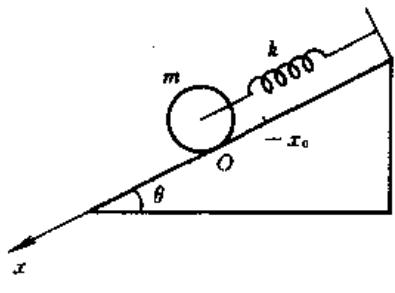
\includegraphics[width=0.2\textwidth]{figures/力图7-5-1.jpg}
\end{center}
\vfill

\textbf{7-6} 【题6】如力图7-6-1，直角形均匀细杆的水平杆长为 $l$ 、质量为 $m$ ，竖直杆长为 $2l$ 、质量为 $2m$ ，细杆可绕拐角处的固定轴 $\mathcal{O}$ 无摩擦地转动．水平杆的一端与劲度系数为 $k$ 的弹簧相连，平衡时水平杆呈水平状态,竖直杆竖直下垂.试求微小摆动的周期.

\begin{center}
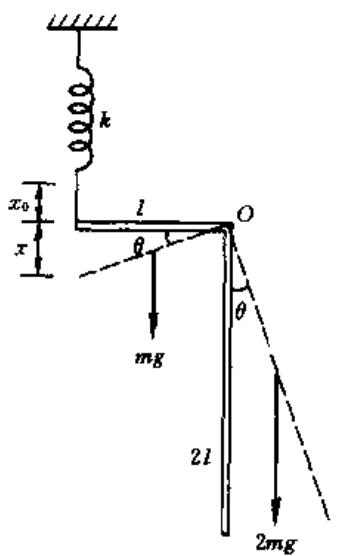
\includegraphics[width=0.2\textwidth]{figures/力图7-6-1.jpg}
\end{center}
\vfill

\newpage
\textbf{7-7} 【题7】如力图7-7-1, 弹簧振子中的小球质量为 $M$ , 弹簧的劲度系数为 $k$ , 弹簧的质量不可忽

略,设为 m, 假定弹簧的质量分布均匀, 忽略摩擦力. 试求振动周期.

\begin{center}
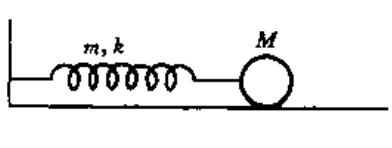
\includegraphics[width=0.3\textwidth]{figures/力图7-7-1.jpg}
\end{center}
\vfill

\textbf{7-8} 【题8】如力图7-8-1，一不可伸长的细线穿过光滑桌面上的小孔，一端系质量为 $m$ 的小球，另一端系质

量为 M 的重物．小球在桌面上以角速度 $\omega_{0}$ 作匀速圆周运动，重物静止不动．若重物受到竖直向上或向下的扰动．试证明，重物将作上、下的简谐振动，并求振动圆频率．

\begin{center}
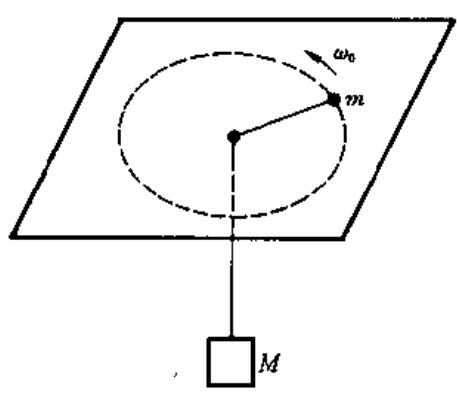
\includegraphics[width=0.25\textwidth]{figures/力图7-8-1.jpg}
\end{center}
\vfill

\newpage
\textbf{7-9} 【题9】如力图7-9-1，光滑的水平平板绕铅垂轴 $Oz$ 逆时针作匀角速转动，角速度为 $\omega$ 。在板面上，一质量可略、原长为 $l$ 、劲度系数为 $k$ 的弹簧一端固定在 $O$ 点，另一端系一质量为 $m$ 的小球。开始时小球位于 $(x_0,0)$ ，初速度为 $(v_0,0)$ 。试求小球相对平板的运动方程 $x = x(t), y = y(t)$ 。

\begin{center}
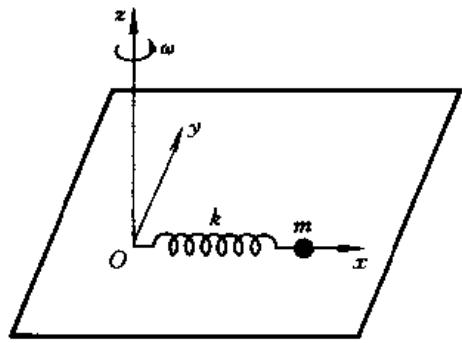
\includegraphics[width=0.2\textwidth]{figures/力图7-9-1.jpg}
\end{center}
\vfill

\textbf{7-10} 【题10】在有些湖中，有时可观察到一种奇妙的湖震现象（水振荡）。通常是在一个浅的，长而比较窄的湖里可以看到。好像水的整体在运动，像你拿着一杯咖啡送到客人那里去时那样。不能把这种现象当作湖面上的水波。

我们用一只矩形容器作模型．容器的长度为 L，水高为 h．假定水面开始时与水平面成一小角度．水面开始振荡，振荡时水面仍保持平面，只是绕位于容器长度一半处的水平轴作振荡．

1. 试建立水运动的模型, 并求出振荡周期 $T$ 的表达式. 初始条件在力图7-10-1中给出. 假定 $\xi \ll h$ .

2. 下面两个表显示在两种不同长度的容器中, 不同深度的水

的振荡时间．以适当的方法检查你得出的公式,看它是否与实验数据很好吻合,并说明你对这种物理模型的适用性的意见．

表 1 L = 479 mm

<table><tr><td>h/mm</td><td>T/s</td></tr><tr><td>30</td><td>1.78</td></tr><tr><td>50</td><td>1.40</td></tr><tr><td>69</td><td>1.18</td></tr><tr><td>88</td><td>1.08</td></tr><tr><td>107</td><td>1.00</td></tr><tr><td>124</td><td>0.91</td></tr><tr><td>142</td><td>0.82</td></tr></table>

表 2 L = 143 mm

<table><tr><td>h/mm</td><td>T/s</td></tr><tr><td>31</td><td>0.52</td></tr><tr><td>38</td><td>0.48</td></tr><tr><td>58</td><td>0.43</td></tr><tr><td>67</td><td>0.35</td></tr><tr><td>124</td><td>0.28</td></tr></table>

3. 力图 7-10-2 所示是在瑞典的 Vattern 湖上测量的结果, 两条曲线分别代表在湖的北端

Bastedalen 和南端 Jönköping 的测量．该湖长度为 123 km，平均深度为 50 m．在此情况下，时间标度应是什么？

\begin{center}
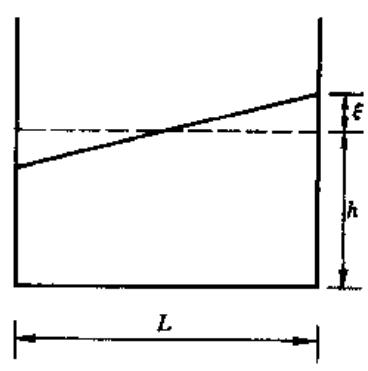
\includegraphics[width=0.3\textwidth]{figures/力图7-10-1.jpg}
\end{center}
\vfill

\newpage
\textbf{7-11} 【题11】如力图7-11-1，质量为 $m_{1}$ 的滑块可在光滑水平直导轨上滑动，滑块经长为 $l$ 质量可略的细杆

与质量为 $m_{2}$ 的重锤相连，细杆与重锤可绕滑块无摩擦地自由转动。设 $t = 0$ 时，细杆与导轨构成铅垂面，细杆与铅锤线夹角 $\theta_0$ ，从静止释放开始摆动。试求：1. 重锤 $m_{2}$ 的运动轨迹。2. 系统作小角摆动时，滑块位置随时间的变化。

\begin{center}
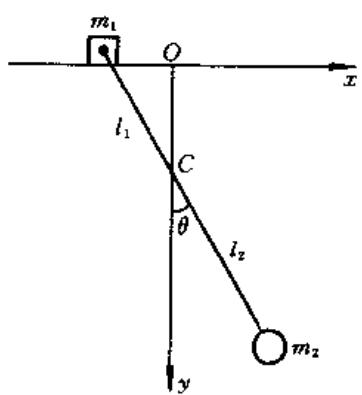
\includegraphics[width=0.2\textwidth]{figures/力图7-11-1.jpg}
\end{center}
\vfill

\textbf{7-12} 【题12】如力图7-12-1,质量为 $m$ , 半径为 $r$ 的均匀实心小球在半径为 $R$ 的球形碗底作纯滚动. 试求微小振动的周期.

\begin{center}
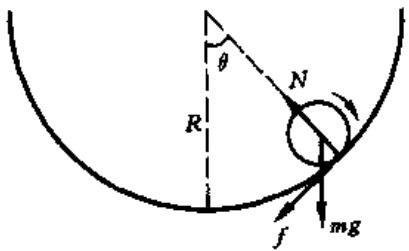
\includegraphics[width=0.2\textwidth]{figures/力图7-12-1.jpg}
\end{center}
\vfill

\newpage
\textbf{7-13} 【题13】如力图7-13-1, 质量为 $M$ 的物体放置在两个完全相同的质量均为 $m$ 的薄壁中空圆筒上. 物体两侧系着两个完全相同的劲度系数均为 $k$ 的弹簧, 两弹簧的另一端固定, 开始时两弹簧均为原长. 设物体在两薄圆筒上作纯滚动. 试求振动圆频率.

\begin{center}
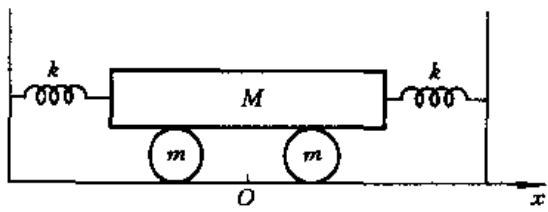
\includegraphics[width=0.3\textwidth]{figures/力图7-13-1.jpg}
\end{center}
\vfill

\textbf{7-14} 【题14】如力图7-14-1，圆盘绕通过中心 $O$ 点的竖直轴在水平面内匀速转动，角速度为 $\omega$ ，质量为 $m$ 的小球被约束在圆盘上的光滑导轨 $AB$ 内运动。小球与一劲度系数为 $k$ 的弹簧相连 $(k > m\omega^2)$ ，弹簧另一端固定在圆盘 $A$ 点。弹簧为原长时，小球位于 $P$ 点， $OP = r_0$ ，且 $OP \perp AB$ ，将小球从 $P$ 点沿导轨拉开距离 $a$ 后从静止释放。在圆盘参考系中考察小球的运动。

1. 试求小球的平衡位置.2. 试证明小球作简谐振动,并求圆频率.3. 试求导轨施予小球的水平力随时间的变化规律.4. 试问当 $k < m\omega^2$ 时小球怎样运动.

\begin{center}
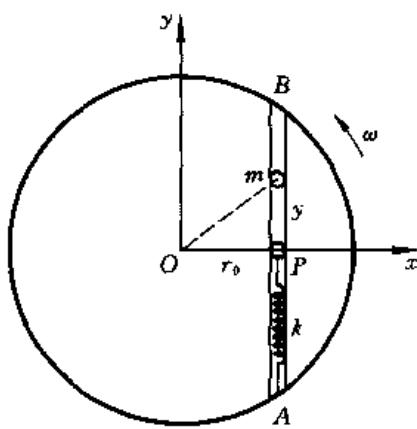
\includegraphics[width=0.2\textwidth]{figures/力图7-14-1.jpg}
\end{center}
\vfill

\newpage
\textbf{7-15} 【题15】如力图7-15-1，质量为 $m$ 的小球在光滑水平桌面上以角速度 $\omega$ 作匀速圆周运动。所需的向心力由与小球相连的弹簧提供，弹簧的劲度系数为 $k$ ，另一端固定。今沿径向轻击小球。试求小球径向振动的频率。

\begin{center}
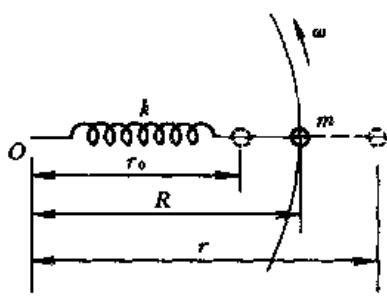
\includegraphics[width=0.2\textwidth]{figures/力图7-15-1.jpg}
\end{center}
\vfill

\textbf{7-16} 【题16】计算单摆周期时，若摆幅 $\theta_0$ 较小，可采用一级近似 $\sin \theta \approx \theta$ ，算出的周期为 $T_{0} = 2\pi \sqrt{\frac{l}{g}}$ ，其中 $l$ 为摆长。若 $\theta_0$ 不算小，就应取二级近似。试导出单摆周期 $T$ 与摆幅 $\theta_0$ 的关系。
\vfill

\newpage
\textbf{7-17} 【题17】对于谐振子, 若广义动量为 $p$ , 广义坐标为 $q$ , 则有 $\oint p \mathrm{d} q = \frac{E}{\nu}$ , 其中 $E$ 为谐振子的能量, $\nu$ 为振动频率. 积分在振动的一个周期内进行. 试就弹簧振子和单摆的情况证明此式.
\vfill

\textbf{7-18} 【题18】如力图7-18-1, $T$ 形导轨固定在铅垂面内, 质量为 $m$ 、全长为 $l$ 的刚性均匀细杆两端约束在 $T$ 形导轨中, 可沿导轨作无摩擦的滑动. 1. 试求细杆作小振幅摆动时的振动周期. 2. 当细杆摆至右方适当角度刚好达到静止时 (如力图7-18-1中虚线所示), 一质量也为 $m$ 的小球以速度 $v_{0}$ 沿水平方向经导轨与细杆上端相碰. 设碰撞无机械能损失, 碰后小球速度变为零, 细杆则回摆到左方与水平导轨平行时刚好静止. 试问 $v_{0}$ 应为多大?

\begin{center}
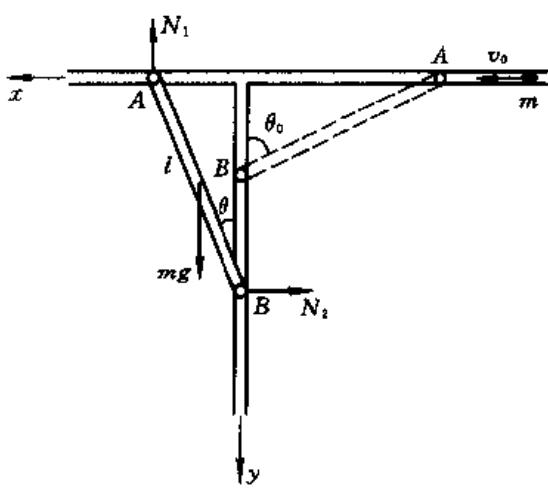
\includegraphics[width=0.25\textwidth]{figures/力图7-18-1.jpg}
\end{center}
\vfill

\newpage
\textbf{7-19} 【题19】如力图7-19-1，在光滑水平面上，质量为 $m_{1}$ 和 $m_{2}$ 的两物体用劲度系数为 $k$ 的弹簧相连。当弹簧为原长时， $m_{1}$ 与 $m_{2}$ 相距 $l_{0}$ ，把弹簧压缩距离 $a$ 后从静止释放。试求 $m_{1}$ 和 $m_{2}$ 的振动表达式。

\begin{center}
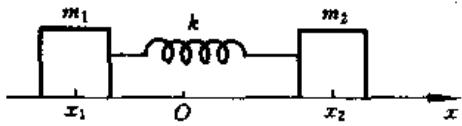
\includegraphics[width=0.3\textwidth]{figures/力图7-19-1.jpg}
\end{center}
\vfill

\textbf{7-20} 【题20】如力图7-20-1，单摆的原长为 $l_{0}$ ，在摆动过程中缓慢上拉，悬点位置不变而摆长逐渐缩短。试求

当摆长缩短为原长之半，即 $l = \frac{l_0}{2}$ 时的振幅与原振幅之比。

\begin{center}
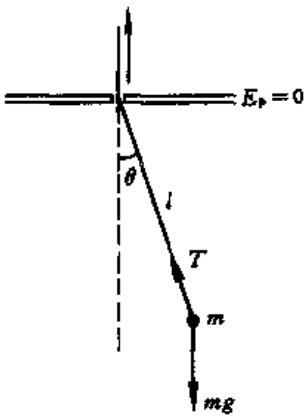
\includegraphics[width=0.2\textwidth]{figures/力图7-20-1.jpg}
\end{center}
\vfill

\newpage
\textbf{7-21} 【题21】如力图7-21-1，质量为 $M$ 、长为 $L$ 的均匀刚性细杆的一端悬挂，可在铅垂面内绕悬点无摩擦地

摆动．质量为 $m=\frac{M}{3}$ 的小虫相对杆以速度 $v_{s}$ 缓慢地沿杆向下爬行．开始时，杆静止并与竖直线夹 $\theta_{0}$ 角（设 $\theta_{0}$ 很小）；小虫位于杆上端的悬点．放开后，杆开始摆动，小虫开始爬行．

试求:1. 小虫沿杆爬行 l 距离时,杆摆动的圆频率.2. 小虫爬到杆下端时,杆摆动的幅度.

\begin{center}
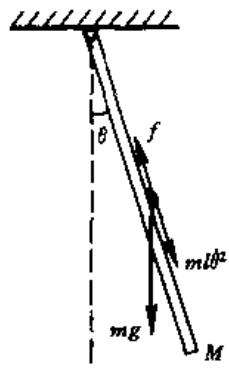
\includegraphics[width=0.15\textwidth]{figures/力图7-21-1.jpg}
\end{center}
\vfill

\textbf{7-22} 【题22】如力图7-22-1，圆盘在水平面内以匀角速 $\Omega$ 绕竖直轴 $OO'$ 旋转，盘上固连着两根同样高度的竖直支架。质量为 $m$ 的小球与质量可忽略不计的 $T$ 字形细杆相连，水平杆由支架支承，与小球相连的杆长为 $l$ ，悬点 $O'$ 在转轴上，整个系统可在支架上无摩擦地摆动。

试求:1. 小球的平衡位置.2. 小球作小幅摆动时的圆频率.

\begin{center}
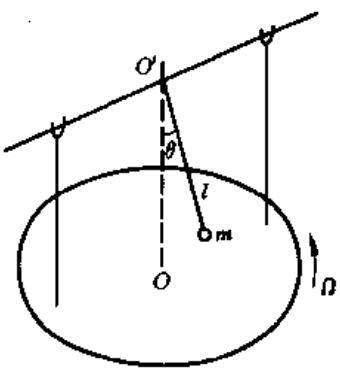
\includegraphics[width=0.2\textwidth]{figures/力图7-22-1.jpg}
\end{center}
\vfill

\newpage
\textbf{7-23} 【题23】如力图7-23-1，在光滑水平面上有三质点 $A, B, C$ ，质量分别为 $m_1, m_2$ 和 $m_3$ ，三质点位于同一直线上，开始时 $B$ 和 $C$ 静止，用劲度系数为 $k$ 的弹簧（质量忽略）相连。质点 $A$ 以初速 $v_0$ 沿连线方向与 $B$ 作完全弹性碰撞。



1. 以 $A$ 和 $B$ 的碰撞点为坐标原点, 连线为 $x$ 轴, 试求碰后质点 $B$ 的运动规律. 2. 设 $m_2 = m_3 = m$ , 为使质点 $A$ 和 $B$ 在碰后重新相遇, 但不相碰 (即相遇时速度相同), 试问比值 $\frac{m_1}{m}$ 应为多少?

\begin{center}
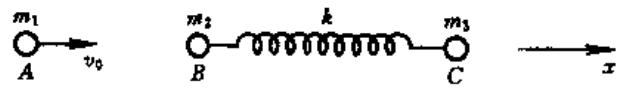
\includegraphics[width=0.35\textwidth]{figures/力图7-23-1.jpg}
\end{center}
\vfill

\textbf{7-25} 【题25】如力图7-25-1，质量为 $m$ 、长为 $l$ 的均匀长方形木板由劲度系数分别为 $k_{1}$ 和 $k_{2}$ 的两竖直弹簧在两端支撑，平衡时木板位于水平面。试求木板作小幅振动时的特征频率。

\begin{center}
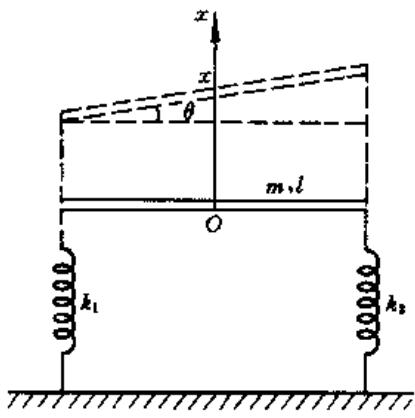
\includegraphics[width=0.25\textwidth]{figures/力图7-25-1.jpg}
\end{center}
\vfill

\newpage
\textbf{7-26} 【题26】如力图7-26-1,两个完全相同的单摆并排悬挂,摆球质量均为 $m$ ,摆长均为 $l$ ,两摆球用劲度系数为 $k$ 的轻质弹簧连接,弹簧原长等于两悬点之间的距离.忽略空气阻力.上述振

动系统称为耦合摆．在小角摆动的条件下，1. 试求耦合摆的特征频率，并写出两摆球运动方程的一般表达式．2. 试讨论耦合摆在不同初始条件下的几种典型运动情况．

\begin{center}
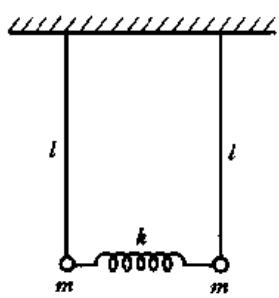
\includegraphics[width=0.2\textwidth]{figures/力图7-26-1.jpg}
\end{center}
\vfill

\textbf{7-27} 【题27】如力图7-27-1，6个质量均为 $m$ 的小球串在光滑圆环上，彼此间用劲度系数均为 $k$ 的6个弹簧相连，整个系统在水平面内。当各小球处在平衡位置时，弹簧均为原长。试求特征频率。

\begin{center}
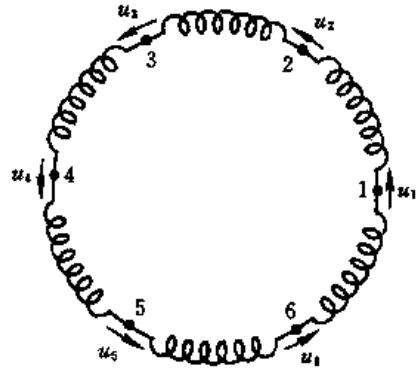
\includegraphics[width=0.2\textwidth]{figures/力图7-27-1.jpg}
\end{center}
\vfill

\newpage
\textbf{7-28} 【题28】三个质量各为 $m$ 的质点由未伸长的无质量弹簧连接在一起达到平衡。每个弹簧的劲度系数为 $k$ ，它们被限制在圆周上运动，如力图7-28-1所示。

1. 若每一质点 $m$ 分别有偏离平衡位置的小位移 $u_{1}, u_{2}$ 和 $u_{3}$ , 试写出每一质点的运动方程

2. 试验证此系统有下列简谐式解
$$
u _ {n} = a _ {n} \cos \omega t
$$
其加速度为 $-\omega^2 u_n$ ，此处 $a_n (n = 1,2,3)$ 是恒振幅，角频率 $\omega$ 有下列三个可能的取值，即
$$
\sqrt {3} \omega_ {0}, \sqrt {3} \omega_ {0}, 0
$$
其中 $\omega_{0}^{2}=\frac{k}{m}$ .

3. 将这由弹簧与质点交替连接的系统扩充到 N 个质点，每一质点 m 由弹簧与相邻质点连接。起初弹簧未伸长，处于平衡，当质点偏离平衡时，用第 n 个质点的位移和相邻质点的位移表示出第 n 个质点 $(n=1,2,\cdots,N)$ 的运动方程。试验证
$$
u _ {n} (t) = a _ {s} \sin \left(\frac {2 n s \pi}{N} + \varphi\right) \cos \omega_ {s} t
$$
是振荡解，式中 $s=1,2,\cdots,N,n=1,2,\cdots,N,\varphi$ 为一任意相位，角频率 $\omega_{s}$ 由下式给出
$$
\omega_ {s} = 2 \omega_ {0} \sin \left(\frac {s \pi}{N}\right)
$$
而 $a_{s}(s=1,2,\cdots,N)$ 是与 n 无关的恒振幅。

试叙述对于一个含有无穷多个质点的链条,频率的可能范围.

4. 试确定 $\frac{u_n}{u_{n+1}}$ 的比值。

当 $N$ 很大时, 对于下列 $(a), (b)$ 两种情况, 试画出说明时刻 $t$ 质点的位移与该质点在链上编号之间关系的草图.

(a)低频解.

$(b)\omega_{s}=\omega_{\max}$ ，其中 $\omega_{\max}$ 是最大的频率解。

5. 若质点之一用质量 $m^{\prime} \ll m$ 的质点代替, 试估计角频率分布将发生怎样的主要变化.

试在上面结果的基础上定性地描述,由质量为 m 和 $m'$ 交替联接的双原子链会有怎样形式的频谱.

提示：
$$
\begin{array}{r l} \sin (A + B) & = \sin A \cos B + \cos A \sin B \\ \sin A + \sin B & = 2 \sin \frac {A + B}{2} \cos \frac {A - B}{2} \\ 2 \sin^ {2} A & = 1 - \cos 2 A \end{array}
$$

\begin{center}
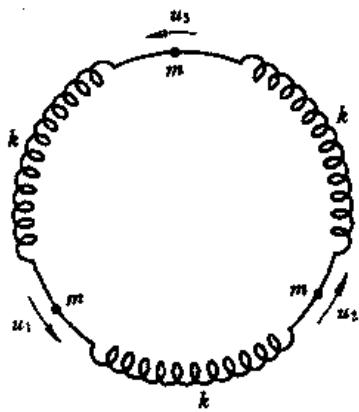
\includegraphics[width=0.2\textwidth]{figures/力图7-28-1.jpg}
\end{center}
\vfill
\newpage

\textbf{7-29} 【题29】如力图7-29-1，细杆长 $l$ ，上端 $O$ 悬挂，下端与质量为 $m$ 的摆球相连，摆球可绕 $O$ 轴无摩擦地摆动。今在细杆的 $A$ 点经连杆接一阻尼器，阻尼力 $f$ 沿水平方向，其大小

与阻尼板的速度 $v$ 成正比，即 $f = \gamma v, \gamma$ 为阻力系数。设 $OA = a$ ，细杆、连杆、阻尼板等的质量均远小于 $m$ ，可忽略不计，阻尼较弱。试求小幅阻尼振动的对数减缩，以及一周期内损失能量的百分比。

\begin{center}
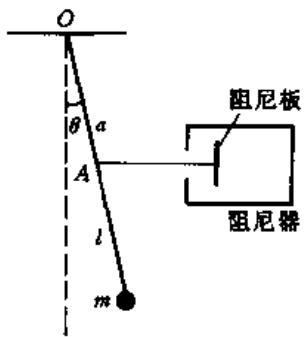
\includegraphics[width=0.2\textwidth]{figures/力图7-29-1.jpg}
\end{center}
\vfill


\textbf{7-30} 【题30】质量为 $m$ 的质点在弹性力和阻尼力的作用下沿 $x$ 轴运动。取平衡位置为坐标原点，弹性力为 $-kx$ ，阻尼力为 $-\gamma x$ 。试问，是否在临界阻尼情况下，质点回到平衡位置一定最快？
\vfill
\newpage


\textbf{7-31} 【题31】如力图7-31-1，充满液体的容器在竖直方向上下振动，质量为 $m$ 的重物由劲度系数为 $k$ 的弹簧悬挂，浸没在液体之中。设悬点随容器振动的规律为 $x_{H} = A\cos \omega t$ ，设液体的阻尼系数为 $\gamma$ （弱阻尼），并假定液体的浮力恒定。

1. 若 $\omega = \omega_0$ ，试求稳定后重物的振动表达式，其中 $\omega_0 = \sqrt{\frac{k}{m}}$ 为弹簧振子的固有圆频率。

2. 若 $\omega \gg \omega_0$ ，试求稳定后重物的振动表达式。

3. 若 $\omega \gg \omega_{0}$ ，且当容器达到最高点时突然停止不动，试求此后重物的振动表达式。

4. 试画出容器突然停止以前和以后的振动曲线。

\begin{center}
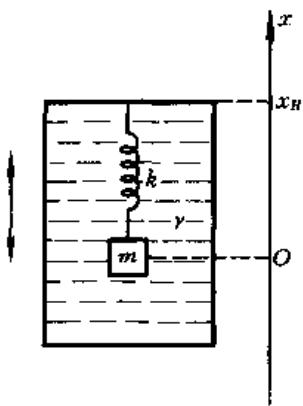
\includegraphics[width=0.2\textwidth]{figures/力图7-31-1.jpg}
\end{center}
\vfill


\textbf{7-32} 【题32】如力图7-32-1，质量均为 $m$ 的三个滑块放置在光滑水平桌面上，彼此以原长为 $x_0$ 、劲度系数为

k 的二个相同弹簧连接起来。开始时三滑块静止，滑块 A 位于原点 O，两弹簧均为原长。对滑块 A 施以周期性外力 F，已知 $F = F_{0} \cos \omega t$ ，在水平方向并沿三滑块连线。试求振动系统的特征频率，并写出滑块 C 的运动方程。

\begin{center}
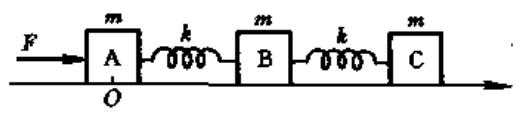
\includegraphics[width=0.3\textwidth]{figures/力图7-32-1.jpg}
\end{center}
\vfill
\newpage

\textbf{7-33} 【题33】本世纪初曾提出一种地球模型，认为它是一个半径为 $R$ 的球体，从地球表面向内到半

径 $R_{C}$ 处为均匀各向同性的固态地幔， $R_{C}$ 以内的地芯为液态，如力图 7-33-1 所示。

在地幔内,地震纵波 p 和横波 s 的速度分别为常量 $v_{p}$ 和 $v_{s}$ ; 在地芯内,纵波的速度为常量 $v_{Cp}$ , 且 $v_{Cp} < v_{p}$ , 而横波不传播.

在地球表面 E 处发生了一次地震, 产生的地震波在地球内传播, 且被地球表面 X 处设置有地震仪的观察者观察到 .E 点和 X 点的角间隔 $2\theta = \angle EOX$ , 其中 O 为地球中心.

1. 试证明, 对于 $\theta \leqslant \arccos \frac{R_C}{R}$ 的那些 $X$ 点, 从 $E$ 点发出的地震波沿直线穿过地幔传播到 $X$ 点的时间为 $t = \frac{2R\sin\theta}{v}$ , 对于 $p$ 波, $v = v_p$ , 对于 $s$ 波 $v = v_s$ .

2. 对于 $\theta > \arccos \frac{R_C}{R}$ 的那些 $X$ 点，地震 $p$ 波在地幔和地芯的界面上经过两次折射后到达 $X$ 点。画出这种地震 $p$ 波的传播路径，并求出对于 $p$ 波， $\theta$ 和 $i$ 之间的关系式，这里 $i$ 是 $p$ 波在地幔和地芯界面上的入射角。

3. 利用下列数据和第2问中所得结果，画出 $\theta \sim i$ 图形. $R = 6370\mathrm{km}, R_C = 3470\mathrm{km}, v_p = 10.85\mathrm{km/s}, v_s = 6.31\mathrm{km/s}, v_{Cp} = 9.02\mathrm{km/s}$ . 试评论，对于地球表面不同地点的观察者，从上述 $\theta \sim i$ 图形可得出什么物理结论.

4. 在一次地震后, 某观察者测出 $s$ 波相对 $p$ 波的时间延迟为 2 分 11 秒, 试用第 3 问中给出的数据确定地震地点与观察者之间的角间隔.

5. 在上述测量中, 观察者注意到某次 $p$ 波和 $s$ 波到达后, 地震仪上还有两个相间 6 分 37 秒的记录. 试解释这一结果, 并验证这与第 4 问所得的角间隔确实相符.
\vfill
\newpage


\textbf{7-34} 【题34】到晚上,地面辐射降温使空气层产生温度梯度,温度随高度递增,这导致声速 $v$ 随高度 $y$ 变化.假定变化规律为

$$
v = v _ {0} (1 + a ^ {2} y ^ {2})
$$

式中 $v_{0}$ 是地面 $(y = 0)$ 处的声速， $\alpha$ 为比例系数。今远方地面上某声源发出一束声波，发射方向与竖直方向成 $\theta_{0}$ 角。假定在声波传播范围内 $\alpha y \ll 1$ 。试导出该束声波在空间传播所循的轨迹，并求地面上听得最清晰的地点与声源的距离。
\vfill
\newpage

\textbf{7-35} 【题35】在海洋中，声波的速度随深度、温度和含盐量变化。已知声速随深度变化的规律如力图7-35-1所示。最小声速 $v_{0}$ 出现在海洋表面和海底之间，以最小声速处作为坐标原点， $z_{s}$ 和 $z_{b}$ 分别表示海洋表面和海底的坐标，则声速v与z的关系为

$$
v = \left\{ \begin{array}{l l} v _ {0} + b z & (z > 0) \\ v _ {0} & (z = 0) \\ v _ {0} - b z & (z <   0) \end{array} \right.
$$

其中 $b$ 为正的常量.

如力图7-35-2，今在 $x = 0, z = 0$ 处放置一声源 $S$ 。在 $zx$ 平面内，从 $S$ 发出的声波的传播方向用初始发射角 $\theta_0$ 表示。声速的不均匀将导致波射线的弯曲。

1. 试证明在 $zx$ 平面内声波的初始轨迹是半径为 $R$ 的圆弧，且

$$
R = \frac {v _ {0}}{b \sin \theta_ {0}} \quad \left(0 \leqslant \theta_ {0} <   \frac {\pi}{2}\right)
$$

2. 在不被海洋表面反射的声波中, 最小的 $\theta_{0}$ 是什么?

3. 设在 Ox 轴上 x = X 处设置接收器 H，试导出能直接到达接收器的各声波所对应的 $\theta_{0}$ 的公式。（排除经海洋表面和海底而到达接收器的情形。）

4. 已知 $X = 10000 \mathrm{~m}, v_0 = 1500 \mathrm{~m/s}, b = 0.020 \mathrm{~s}^{-1}$ . 试用这些数据计算可使声波直接从 $S$ 传到 $H$ (不经反射) 的 4 个 $\theta_0$ 的值 (从最小的 $\theta_0$ 开始).

5. 当 $\theta_0$ 取第3问中得出的最小值时, 试导出声波从 $S$ 传播到 $H$ 所需时间的表达式, 并用第4问所给的数据算出这个传播时间. 再计算当 $\theta_0 = \frac{\pi}{2}$ 时, 即声波沿 $x$ 传播到 $H$ 所需的时间. 比较上述两个时间的大小.

\begin{center}
    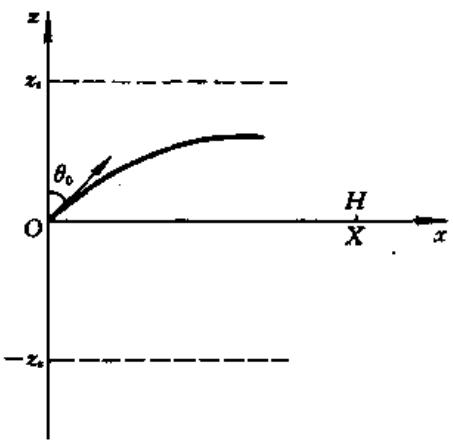
\includegraphics[width=0.2\textwidth]{figures/力图7-35-2.jpg}
    \quad
    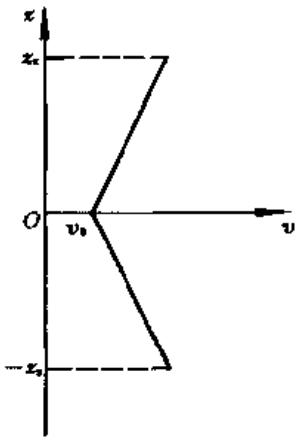
\includegraphics[width=0.15\textwidth]{figures/力图7-35-1.jpg}
\end{center}

\vfill

\newpage


\textbf{7-36} 【题36】如力图7-36-1,质量为 $m$ 、劲度系数为 $\pmb{k}$ 的弹簧原长为 $L$ ,一端固定,另一端与一质量为 $M$ 的物体相连,整个系统水平放置,物体 $M$ 可在光滑水平面上滑动.1.试导出纵向弹性波的波动方程并求波速.2.假定 $L$ 远小于弹性波的波长, $M$ 的振幅为 $A_0$ ,试求弹簧上各点的振幅分布.3.在 $m \ll M$ 的条件下,试分别求零级近似和一级近似的频率.

\begin{center}
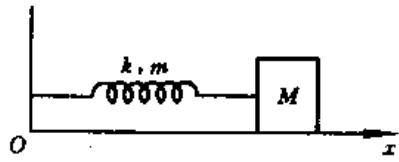
\includegraphics[width=0.3\textwidth]{figures/力图7-36-1.jpg}
\end{center}
\vfill

\textbf{7-37} 【题37】无穷长弦线，拉紧，质量线密度为 $\rho = 0.01\mathrm{kg / m}$ 。今在线一端施以横向简谐力，峰值为 $F_{\max} = 0.3\mathrm{N}$ ，使弦线中产生简谐振动，波速为 $v = \frac{30}{\pi}\mathrm{m / s}$ 。试求单位时间内通过弦线某一截面传输的平均能量 $S$ 。
\vfill

\newpage
\textbf{7-38} 【题38】拉紧的弦线，张力为 $T$ ，质量线密度为 $\rho$ ，质量为 $m$ 的质点附在弦上某点．圆频率为 $\omega$ 的波沿弦线传播．试求波在质点 $m$ 反射时的能量反射系数．
\vfill

\textbf{7-39} 【题39】音叉与频率为 $250.0\mathrm{Hz}$ 的标准声源同时发音时，产生 $1.5\mathrm{Hz}$ 的拍音。当音叉粘上一小块橡皮泥时，拍频增加了。如力图7-39-1，将该音叉放在盛水的细管口，连续调节水面的高度，当空气柱高度相继为 $0.34\mathrm{m}$ 和 $1.03\mathrm{m}$ 时发生共振。

试求:

1. 声波在空气中的声速.

2. 画出空气柱中的驻波图.

\begin{center}
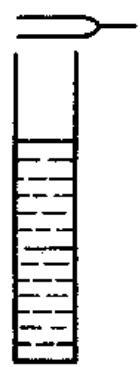
\includegraphics[width=0.1\textwidth]{figures/力图7-39-1.jpg}
\end{center}
\vfill

\newpage
\textbf{7-40} 【题40】小提琴弦长为 $L$ ，质量线密度为 $\rho$ ，张力为 $T.1$ 。用手指轻按弦的中点，试求基频和一次谐波的频率，并写出弦上各点的振动方程式。2. 在弦的一端 $\frac{L}{3}$ 长度上均匀包缠细线，使其线密度增加为 $4\rho$ ，放开手指，试求基频，并写出弦上各点的振动表达式。
\vfill\newpage

\textbf{7-41} 【题41】一列振幅为 $A$ ，频率为 $\nu$ ，波长为 $\lambda$ 的横波沿一拉紧的水平细线传播。细线单位长度的质量为 $\rho$ 。任一点位移的表达式为
$$
y _ {1} = A \sin 2 \pi \left(\nu t - \frac {x}{\lambda}\right)
$$

式中 $t$ 为时间, $x$ 为细线上各点的水平坐标.

另一列具有相同振幅、频率、波长的波同时在细线中沿相反方向传播。两列波 $t = 0$ 时在 $x = 0$ 处的相位差为 $\varphi$ 。今在 $x = 0$ 和 $x = L$ 两处将细线固定。

1. 试导出细线中的驻波方程，并求细线中所有可能存在的波长。

2. 试求任意时刻的总动能和总势能，规定细线上各点均处于平衡位置时的总势能为零点。

3. 设 $L = 2.50 \mathrm{~m}$ , 长为 $L$ 的细线的质量为 $m = 0.0100 \mathrm{~kg}$ , 细线中的张力 $T = 10.0 \mathrm{~N}$ , 驻波的最大振幅为 $0.02 \mathrm{~m}$ . 

(a) 试求基模的频率和对应的总能量. 

(b) 用手拨动细线, 在其中激起所有可能的驻波模式, 然后在距端点 $0.50 \mathrm{~m}$ 处抓住细线. 试问哪些频率的驻波可在细线中继续存留.



\vfill
\newpage



\textbf{7-42}  【题42】飞机在上空以速度 $v = 200\mathrm{m / s}$ 作水平飞行，发出频率为 $\nu_{0} = 2000\mathrm{Hz}$ 的声波。静止在地面上的观察者测定飞机发出的声波的频率，当飞机越过观察者上空时，观察者在 $4\mathrm{s}$ 钟内测出的频率从 $\nu_{1} = 2400\mathrm{Hz}$ 降为 $\nu_{2} = 1600\mathrm{Hz}$ 。已知声波在空气中的速度为 $v = 330\mathrm{m / s}$ ，试求飞机的飞行高度 $h$ 。

\vfill





\textbf{7-43}  【题43】如图，音叉 $P$ 沿着半径 $r = 8\mathrm{m}$ 的圆以角速度 $\omega = 4\mathrm{rad / s}$ 作匀速圆周运动。音叉发出频率为 $\nu_{0} = 500\mathrm{Hz}$ 的声波，声波的速度为 $v = 330\mathrm{m / s}$ 。观测者 $M$ 与圆周共面，与圆心 $O$ 的距离为 $d = 2r$ 。试问当 $\theta$ 角为多大时，观测到的频率为最高或最低，并求其数值。 $\theta$ 是 $OP$ 和 $OM$ 的夹角。

\begin{center}
    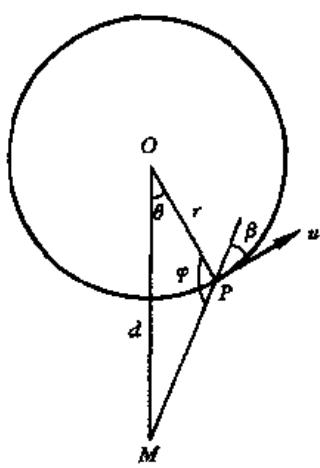
\includegraphics[width = 0.2\textwidth]{figures/力图7-43-1.jpg}
\end{center}

\vfill



